% 1. age
\clearpage
\begin{figure}[!ht]
    \centering
    % figura 1
    \begin{subfigure}[b]{0.48\textwidth}
        \centering
        \includegraphics[width = 8cm, height = 7cm]{old_ti/age.png}
        \caption{Alunos Seniors da FT}
    \end{subfigure}
    ~
    % figura 2
    \begin{subfigure}[b]{0.48\textwidth}
        \centering
        \includegraphics[width = 8cm, height=7cm]{yng_ti/age.png}
        \caption{Alunos Jovens da FT}
    \end{subfigure}

    % figura 3
    \begin{subfigure}[b]{0.48\textwidth}
        \centering
        \includegraphics[width = 8cm, height=7cm]{old_lic/age.png}
        \caption{Alunos Seniors da Licenciatura}
    \end{subfigure}
    ~
    % figura 4
    \begin{subfigure}[b]{0.48\textwidth}
        \centering
        \includegraphics[width = 8cm, height=7cm]{yng_lic/age.png}
        \caption{Alunos Jovens da Licenciatura}
    \end{subfigure}

    % figura 5
    \begin{subfigure}[b]{0.48\textwidth}
        \centering
        \includegraphics[width = 8cm, height=7cm]{old_comp/age.png}
        \caption{Alunos Seniors da Computação}
    \end{subfigure}
    ~
    % figura 6
    \begin{subfigure}[b]{0.48\textwidth}
        \centering
        \includegraphics[width = 8cm, height=7cm]{yng_comp/age.png}
        \caption{Alunos Jovens da Computação}
    \end{subfigure}
    \caption{Atributo Idade, conforme os diferentes modelos}
\end{figure}

% 2. course
\clearpage
\begin{figure}[!ht]
    \centering
    % figura 1
    \begin{subfigure}[b]{0.48\textwidth}
        \centering
        \includegraphics[width = 8cm, height = 7cm]{old_ti/course.png}
        \caption{Alunos Seniors da FT}
    \end{subfigure}
    ~
    % figura 2
    \begin{subfigure}[b]{0.48\textwidth}
        \centering
        \includegraphics[width = 8cm, height=7cm]{yng_ti/course.png}
        \caption{Alunos Jovens da FT}
    \end{subfigure}

    % figura 3
    \begin{subfigure}[b]{0.48\textwidth}
        \centering
        \includegraphics[width = 8cm, height=7cm]{old_lic/course.png}
        \caption{Alunos Seniors da Licenciatura}
    \end{subfigure}
    ~
    % figura 4
    \begin{subfigure}[b]{0.48\textwidth}
        \centering
        \includegraphics[width = 8cm, height=7cm]{yng_lic/course.png}
        \caption{Alunos Jovens da Licenciatura}
    \end{subfigure}

    % figura 5
    \begin{subfigure}[b]{0.48\textwidth}
        \centering
        \includegraphics[width = 8cm, height=7cm]{old_comp/course.png}
        \caption{Alunos Seniors da Computação}
    \end{subfigure}
    ~
    % figura 6
    \begin{subfigure}[b]{0.48\textwidth}
        \centering
        \includegraphics[width = 8cm, height=7cm]{yng_comp/course.png}
        \caption{Alunos Jovens da Computação}
    \end{subfigure}
    \caption{Atributo Curso, conforme os diferentes modelos}
\end{figure}

% 5. sex
\clearpage
\begin{figure}[!ht]
    \centering
    % figura 1
    \begin{subfigure}[b]{0.48\textwidth}
        \centering
        \includegraphics[width = 8cm, height = 7cm]{old_ti/sex.png}
        \caption{Alunos Seniors da FT}
    \end{subfigure}
    ~
    % figura 2
    \begin{subfigure}[b]{0.48\textwidth}
        \centering
        \includegraphics[width = 8cm, height=7cm]{yng_ti/sex.png}
        \caption{Alunos Jovens da FT}
    \end{subfigure}

    % figura 3
    \begin{subfigure}[b]{0.48\textwidth}
        \centering
        \includegraphics[width = 8cm, height=7cm]{old_lic/sex.png}
        \caption{Alunos Seniors da Licenciatura}
    \end{subfigure}
    ~
    % figura 4
    \begin{subfigure}[b]{0.48\textwidth}
        \centering
        \includegraphics[width = 8cm, height=7cm]{yng_lic/sex.png}
        \caption{Alunos Jovens da Licenciatura}
    \end{subfigure}

    % figura 5
    \begin{subfigure}[b]{0.48\textwidth}
        \centering
        \includegraphics[width = 8cm, height=7cm]{old_comp/sex.png}
        \caption{Alunos Seniors da Computação}
    \end{subfigure}
    ~
    % figura 6
    \begin{subfigure}[b]{0.48\textwidth}
        \centering
        \includegraphics[width = 8cm, height=7cm]{yng_comp/sex.png}
        \caption{Alunos Jovens da Computação}
    \end{subfigure}
    \caption{Atributo Sexo, conforme os diferentes modelos}
\end{figure}

% 6. quota
\clearpage
\begin{figure}[!ht]
    \centering
    % figura 1
    \begin{subfigure}[b]{0.48\textwidth}
        \centering
        \includegraphics[width = 8cm, height = 7cm]{old_ti/quota.png}
        \caption{Alunos Seniors da FT}
    \end{subfigure}
    ~
    % figura 2
    \begin{subfigure}[b]{0.48\textwidth}
        \centering
        \includegraphics[width = 8cm, height=7cm]{yng_ti/quota.png}
        \caption{Alunos Jovens da FT}
    \end{subfigure}

    % figura 3
    \begin{subfigure}[b]{0.48\textwidth}
        \centering
        \includegraphics[width = 8cm, height=7cm]{old_lic/quota.png}
        \caption{Alunos Seniors da Licenciatura}
    \end{subfigure}
    ~
    % figura 4
    \begin{subfigure}[b]{0.48\textwidth}
        \centering
        \includegraphics[width = 8cm, height=7cm]{yng_lic/quota.png}
        \caption{Alunos Jovens da Licenciatura}
    \end{subfigure}

    % figura 5
    \begin{subfigure}[b]{0.48\textwidth}
        \centering
        \includegraphics[width = 8cm, height=7cm]{old_comp/quota.png}
        \caption{Alunos Seniors da Computação}
    \end{subfigure}
    ~
    % figura 6
    \begin{subfigure}[b]{0.48\textwidth}
        \centering
        \includegraphics[width = 8cm, height=7cm]{yng_comp/quota.png}
        \caption{Alunos Jovens da Computação}
    \end{subfigure}
    \caption{Atributo cota, conforme os diferentes modelos}
\end{figure}

% 7. school_type
\clearpage
\begin{figure}[!ht]
    \centering
    % figura 1
    \begin{subfigure}[b]{0.48\textwidth}
        \centering
        \includegraphics[width = 8cm, height = 7cm]{old_ti/school_type.png}
        \caption{Alunos Seniors da FT}
    \end{subfigure}
    ~
    % figura 2
    \begin{subfigure}[b]{0.48\textwidth}
        \centering
        \includegraphics[width = 8cm, height=7cm]{yng_ti/school_type.png}
        \caption{Alunos Jovens da FT}
    \end{subfigure}

    % figura 3
    \begin{subfigure}[b]{0.48\textwidth}
        \centering
        \includegraphics[width = 8cm, height=7cm]{old_lic/school_type.png}
        \caption{Alunos Seniors da Licenciatura}
    \end{subfigure}
    ~
    % figura 4
    \begin{subfigure}[b]{0.48\textwidth}
        \centering
        \includegraphics[width = 8cm, height=7cm]{yng_lic/school_type.png}
        \caption{Alunos Jovens da Licenciatura}
    \end{subfigure}

    % figura 5
    \begin{subfigure}[b]{0.48\textwidth}
        \centering
        \includegraphics[width = 8cm, height=7cm]{old_comp/school_type.png}
        \caption{Alunos Seniors da Computação}
    \end{subfigure}
    ~
    % figura 6
    \begin{subfigure}[b]{0.48\textwidth}
        \centering
        \includegraphics[width = 8cm, height=7cm]{yng_comp/school_type.png}
        \caption{Alunos Jovens da Computação}
    \end{subfigure}
    \caption{Atributo Tipo da Escola, conforme os diferentes modelos}
\end{figure}

% 8. way_in
\clearpage
\begin{figure}[!ht]
    \centering
    % figura 1
    \begin{subfigure}[b]{0.48\textwidth}
        \centering
        \includegraphics[width = 8cm, height = 7cm]{old_ti/way_in.png}
        \caption{Alunos Seniors da FT}
    \end{subfigure}
    ~
    % figura 2
    \begin{subfigure}[b]{0.48\textwidth}
        \centering
        \includegraphics[width = 8cm, height=7cm]{yng_ti/way_in.png}
        \caption{Alunos Jovens da FT}
    \end{subfigure}

    % figura 3
    \begin{subfigure}[b]{0.48\textwidth}
        \centering
        \includegraphics[width = 8cm, height=7cm]{old_lic/way_in.png}
        \caption{Alunos Seniors da Licenciatura}
    \end{subfigure}
    ~
    % figura 4
    \begin{subfigure}[b]{0.48\textwidth}
        \centering
        \includegraphics[width = 8cm, height=7cm]{yng_lic/way_in.png}
        \caption{Alunos Jovens da Licenciatura}
    \end{subfigure}

    % figura 5
    \begin{subfigure}[b]{0.48\textwidth}
        \centering
        \includegraphics[width = 8cm, height=7cm]{old_comp/way_in.png}
        \caption{Alunos Seniors da Computação}
    \end{subfigure}
    ~
    % figura 6
    \begin{subfigure}[b]{0.48\textwidth}
        \centering
        \includegraphics[width = 8cm, height=7cm]{yng_comp/way_in.png}
        \caption{Alunos Jovens da Computação}
    \end{subfigure}
    \caption{Atributo Forma de Entrada, conforme os diferentes modelos}
\end{figure}

% 9. way_out
\clearpage
\begin{figure}[!ht]
    \centering
    % figura 1
    \begin{subfigure}[b]{0.48\textwidth}
        \centering
        \includegraphics[width = 8cm, height = 7cm]{old_ti/way_out.png}
        \caption{Alunos Seniors da FT}
    \end{subfigure}
    ~
    % figura 2
    \begin{subfigure}[b]{0.48\textwidth}
        \centering
        \includegraphics[width = 8cm, height=7cm]{yng_ti/way_out.png}
        \caption{Alunos Jovens da FT}
    \end{subfigure}

    % figura 3
    \begin{subfigure}[b]{0.48\textwidth}
        \centering
        \includegraphics[width = 8cm, height=7cm]{old_lic/way_out.png}
        \caption{Alunos Seniors da Licenciatura}
    \end{subfigure}
    ~
    % figura 4
    \begin{subfigure}[b]{0.48\textwidth}
        \centering
        \includegraphics[width = 8cm, height=7cm]{yng_lic/way_out.png}
        \caption{Alunos Jovens da Licenciatura}
    \end{subfigure}

    % figura 5
    \begin{subfigure}[b]{0.48\textwidth}
        \centering
        \includegraphics[width = 8cm, height=7cm]{old_comp/way_out.png}
        \caption{Alunos Seniors da Computação}
    \end{subfigure}
    ~
    % figura 6
    \begin{subfigure}[b]{0.48\textwidth}
        \centering
        \includegraphics[width = 8cm, height=7cm]{yng_comp/way_out.png}
        \caption{Alunos Jovens da Computação}
    \end{subfigure}
    \caption{Atributo Forma de Saída, conforme os diferentes modelos}
\end{figure}

% 10. credit rate acc
\clearpage
\begin{figure}[!ht]
    \centering
    % figura 1
    \begin{subfigure}[b]{0.48\textwidth}
        \centering
        \includegraphics[width = 8cm, height = 7cm]{old_ti/credit_rate_acc.png}
        \caption{Alunos Seniors da FT}
    \end{subfigure}
    ~
    % figura 2
    \begin{subfigure}[b]{0.48\textwidth}
        \centering
        \includegraphics[width = 8cm, height=7cm]{yng_ti/credit_rate_acc.png}
        \caption{Alunos Jovens da FT}
    \end{subfigure}

    % figura 3
    \begin{subfigure}[b]{0.48\textwidth}
        \centering
        \includegraphics[width = 8cm, height=7cm]{old_lic/credit_rate_acc.png}
        \caption{Alunos Seniors da Licenciatura}
    \end{subfigure}
    ~
    % figura 4
    \begin{subfigure}[b]{0.48\textwidth}
        \centering
        \includegraphics[width = 8cm, height=7cm]{yng_lic/credit_rate_acc.png}
        \caption{Alunos Jovens da Licenciatura}
    \end{subfigure}

    % figura 5
    \begin{subfigure}[b]{0.48\textwidth}
        \centering
        \includegraphics[width = 8cm, height=7cm]{old_comp/credit_rate_acc.png}
        \caption{Alunos Seniors da Computação}
    \end{subfigure}
    ~
    % figura 6
    \begin{subfigure}[b]{0.48\textwidth}
        \centering
        \includegraphics[width = 8cm, height=7cm]{yng_comp/credit_rate_acc.png}
        \caption{Alunos Jovens da Computação}
    \end{subfigure}
    \caption{Atributo Quantidade de Créditos, conforme os diferentes modelos}
\end{figure}

% 11. in condition
\clearpage
\begin{figure}[!ht]
    \centering
    % figura 1
    \begin{subfigure}[b]{0.48\textwidth}
        \centering
        \includegraphics[width = 8cm, height = 7cm]{old_ti/in_condition.png}
        \caption{Alunos Seniors da FT}
    \end{subfigure}
    ~
    % figura 2
    \begin{subfigure}[b]{0.48\textwidth}
        \centering
        \includegraphics[width = 8cm, height=7cm]{yng_ti/in_condition.png}
        \caption{Alunos Jovens da FT}
    \end{subfigure}

    % figura 3
    \begin{subfigure}[b]{0.48\textwidth}
        \centering
        \includegraphics[width = 8cm, height=7cm]{old_lic/in_condition.png}
        \caption{Alunos Seniors da Licenciatura}
    \end{subfigure}
    ~
    % figura 4
    \begin{subfigure}[b]{0.48\textwidth}
        \centering
        \includegraphics[width = 8cm, height=7cm]{yng_lic/in_condition.png}
        \caption{Alunos Jovens da Licenciatura}
    \end{subfigure}

    % figura 5
    \begin{subfigure}[b]{0.48\textwidth}
        \centering
        \includegraphics[width = 8cm, height=7cm]{old_comp/in_condition.png}
        \caption{Alunos Seniors da Computação}
    \end{subfigure}
    ~
    % figura 6
    \begin{subfigure}[b]{0.48\textwidth}
        \centering
        \includegraphics[width = 8cm, height=7cm]{yng_comp/in_condition.png}
        \caption{Alunos Jovens da Computação}
    \end{subfigure}
    \caption{Atributo Em Condição, conforme os diferentes modelos}
\end{figure}

% 12. drop rate
\clearpage
\begin{figure}[!ht]
    \centering
    % figura 1
    \begin{subfigure}[b]{0.48\textwidth}
        \centering
        \includegraphics[width = 8cm, height = 7cm]{old_ti/drop_rate.png}
        \caption{Alunos Seniors da FT}
    \end{subfigure}
    ~
    % figura 2
    \begin{subfigure}[b]{0.48\textwidth}
        \centering
        \includegraphics[width = 8cm, height=7cm]{yng_ti/drop_rate.png}
        \caption{Alunos Jovens da FT}
    \end{subfigure}

    % figura 3
    \begin{subfigure}[b]{0.48\textwidth}
        \centering
        \includegraphics[width = 8cm, height=7cm]{old_lic/drop_rate.png}
        \caption{Alunos Seniors da Licenciatura}
    \end{subfigure}
    ~
    % figura 4
    \begin{subfigure}[b]{0.48\textwidth}
        \centering
        \includegraphics[width = 8cm, height=7cm]{yng_lic/drop_rate.png}
        \caption{Alunos Jovens da Licenciatura}
    \end{subfigure}

    % figura 5
    \begin{subfigure}[b]{0.48\textwidth}
        \centering
        \includegraphics[width = 8cm, height=7cm]{old_comp/drop_rate.png}
        \caption{Alunos Seniors da Computação}
    \end{subfigure}
    ~
    % figura 6
    \begin{subfigure}[b]{0.48\textwidth}
        \centering
        \includegraphics[width = 8cm, height=7cm]{yng_comp/drop_rate.png}
        \caption{Alunos Jovens da Computação}
    \end{subfigure}
    \caption{Atributo Taxa de Trancamento, conforme os diferentes modelos}
\end{figure}

% 13. fail rate
\clearpage
\begin{figure}[!ht]
    \centering
    % figura 1
    \begin{subfigure}[b]{0.48\textwidth}
        \centering
        \includegraphics[width = 8cm, height = 7cm]{old_ti/fail_rate.png}
        \caption{Alunos Seniors da FT}
    \end{subfigure}
    ~
    % figura 2
    \begin{subfigure}[b]{0.48\textwidth}
        \centering
        \includegraphics[width = 8cm, height=7cm]{yng_ti/fail_rate.png}
        \caption{Alunos Jovens da FT}
    \end{subfigure}

    % figura 3
    \begin{subfigure}[b]{0.48\textwidth}
        \centering
        \includegraphics[width = 8cm, height=7cm]{old_lic/fail_rate.png}
        \caption{Alunos Seniors da Licenciatura}
    \end{subfigure}
    ~
    % figura 4
    \begin{subfigure}[b]{0.48\textwidth}
        \centering
        \includegraphics[width = 8cm, height=7cm]{yng_lic/fail_rate.png}
        \caption{Alunos Jovens da Licenciatura}
    \end{subfigure}

    % figura 5
    \begin{subfigure}[b]{0.48\textwidth}
        \centering
        \includegraphics[width = 8cm, height=7cm]{old_comp/fail_rate.png}
        \caption{Alunos Seniors da Computação}
    \end{subfigure}
    ~
    % figura 6
    \begin{subfigure}[b]{0.48\textwidth}
        \centering
        \includegraphics[width = 8cm, height=7cm]{yng_comp/fail_rate.png}
        \caption{Alunos Jovens da Computação}
    \end{subfigure}
    \caption{Atributo Taxa de Falhas, conforme os diferentes modelos}
\end{figure}

% 14. hard rate 
\clearpage
\begin{figure}[!ht]
    \centering
    % figura 1
    \begin{subfigure}[b]{0.48\textwidth}
        \centering
        \includegraphics[width = 8cm, height = 7cm]{old_ti/hard_rate.png}
        \caption{Alunos Seniors da FT}
    \end{subfigure}
    ~
    % figura 2
    \begin{subfigure}[b]{0.48\textwidth}
        \centering
        \includegraphics[width = 8cm, height=7cm]{yng_ti/hard_rate.png}
        \caption{Alunos Jovens da FT}
    \end{subfigure}

    % figura 3
    \begin{subfigure}[b]{0.48\textwidth}
        \centering
        \includegraphics[width = 8cm, height=7cm]{old_lic/hard_rate.png}
        \caption{Alunos Seniors da Licenciatura}
    \end{subfigure}
    ~
    % figura 4
    \begin{subfigure}[b]{0.48\textwidth}
        \centering
        \includegraphics[width = 8cm, height=7cm]{yng_lic/hard_rate.png}
        \caption{Alunos Jovens da Licenciatura}
    \end{subfigure}

    % figura 5
    \begin{subfigure}[b]{0.48\textwidth}
        \centering
        \includegraphics[width = 8cm, height=7cm]{old_comp/hard_rate.png}
        \caption{Alunos Seniors da Computação}
    \end{subfigure}
    ~
    % figura 6
    \begin{subfigure}[b]{0.48\textwidth}
        \centering
        \includegraphics[width = 8cm, height=7cm]{yng_comp/hard_rate.png}
        \caption{Alunos Jovens da Computação}
    \end{subfigure}
    \caption{Atributo taxa de aprovação em disciplinas difíceis, conforme os 
    diferentes modelos}
\end{figure}

% 15. improvement rate
\clearpage
\begin{figure}[!ht]
    \centering
    % figura 1
    \begin{subfigure}[b]{0.48\textwidth}
        \centering
        \includegraphics[width = 8cm, height = 7cm]{old_ti/improvement_rate.png}
        \caption{Alunos Seniors da FT}
    \end{subfigure}
    ~
    % figura 2
    \begin{subfigure}[b]{0.48\textwidth}
        \centering
        \includegraphics[width = 8cm, height=7cm]{yng_ti/improvement_rate.png}
        \caption{Alunos Jovens da FT}
    \end{subfigure}

    % figura 3
    \begin{subfigure}[b]{0.48\textwidth}
        \centering
        \includegraphics[width = 8cm, height=7cm]{old_lic/improvement_rate.png}
        \caption{Alunos Seniors da Licenciatura}
    \end{subfigure}
    ~
    % figura 4
    \begin{subfigure}[b]{0.48\textwidth}
        \centering
        \includegraphics[width = 8cm, height=7cm]{yng_lic/improvement_rate.png}
        \caption{Alunos Jovens da Licenciatura}
    \end{subfigure}

    % figura 5
    \begin{subfigure}[b]{0.48\textwidth}
        \centering
        \includegraphics[width = 8cm, height=7cm]{old_comp/improvement_rate.png}
        \caption{Alunos Seniors da Computação}
    \end{subfigure}
    ~
    % figura 6
    \begin{subfigure}[b]{0.48\textwidth}
        \centering
        \includegraphics[width = 8cm, height=7cm]{yng_comp/improvement_rate.png}
        \caption{Alunos Jovens da Computação}
    \end{subfigure}
    \caption{Atributo Taxa de Melhora Acadêmica, conforme os diferentes modelos}
\end{figure}

% 16. ira
\clearpage
\begin{figure}[!ht]
    \centering
    % figura 1
    \begin{subfigure}[b]{0.48\textwidth}
        \centering
        \includegraphics[width = 8cm, height = 7cm]{old_ti/ira.png}
        \caption{Alunos Seniors da FT}
    \end{subfigure}
    ~
    % figura 2
    \begin{subfigure}[b]{0.48\textwidth}
        \centering
        \includegraphics[width = 8cm, height=7cm]{yng_ti/ira.png}
        \caption{Alunos Jovens da FT}
    \end{subfigure}

    % figura 3
    \begin{subfigure}[b]{0.48\textwidth}
        \centering
        \includegraphics[width = 8cm, height=7cm]{old_lic/ira.png}
        \caption{Alunos Seniors da Licenciatura}
    \end{subfigure}
    ~
    % figura 4
    \begin{subfigure}[b]{0.48\textwidth}
        \centering
        \includegraphics[width = 8cm, height=7cm]{yng_lic/ira.png}
        \caption{Alunos Jovens da Licenciatura}
    \end{subfigure}

    % figura 5
    \begin{subfigure}[b]{0.48\textwidth}
        \centering
        \includegraphics[width = 8cm, height=7cm]{old_comp/ira.png}
        \caption{Alunos Seniors da Computação}
    \end{subfigure}
    ~
    % figura 6
    \begin{subfigure}[b]{0.48\textwidth}
        \centering
        \includegraphics[width = 8cm, height=7cm]{yng_comp/ira.png}
        \caption{Alunos Jovens da Computação}
    \end{subfigure}
    \caption{Atributo IRA, conforme os diferentes modelos}
\end{figure}

% 17. pass rate
\clearpage
\begin{figure}[!ht]
    \centering
    % figura 1
    \begin{subfigure}[b]{0.48\textwidth}
        \centering
        \includegraphics[width = 8cm, height = 7cm]{old_ti/pass_rate.png}
        \caption{Alunos Seniors da FT}
    \end{subfigure}
    ~
    % figura 2
    \begin{subfigure}[b]{0.48\textwidth}
        \centering
        \includegraphics[width = 8cm, height=7cm]{yng_ti/pass_rate.png}
        \caption{Alunos Jovens da FT}
    \end{subfigure}

    % figura 3
    \begin{subfigure}[b]{0.48\textwidth}
        \centering
        \includegraphics[width = 8cm, height=7cm]{old_lic/pass_rate.png}
        \caption{Alunos Seniors da Licenciatura}
    \end{subfigure}
    ~
    % figura 4
    \begin{subfigure}[b]{0.48\textwidth}
        \centering
        \includegraphics[width = 8cm, height=7cm]{yng_lic/pass_rate.png}
        \caption{Alunos Jovens da Licenciatura}
    \end{subfigure}

    % figura 5
    \begin{subfigure}[b]{0.48\textwidth}
        \centering
        \includegraphics[width = 8cm, height=7cm]{old_comp/pass_rate.png}
        \caption{Alunos Seniors da Computação}
    \end{subfigure}
    ~
    % figura 6
    \begin{subfigure}[b]{0.48\textwidth}
        \centering
        \includegraphics[width = 8cm, height=7cm]{yng_comp/pass_rate.png}
        \caption{Alunos Jovens da Computação}
    \end{subfigure}
    \caption{Atributo Taxa de Aprovação, conforme os diferentes modelos}
\end{figure}

% 18. position
\clearpage
\begin{figure}[!ht]
    \centering
    % figura 1
    \begin{subfigure}[b]{0.48\textwidth}
        \centering
        \includegraphics[width = 8cm, height = 7cm]{old_ti/position.png}
        \caption{Alunos Seniors da FT}
    \end{subfigure}
    ~
    % figura 2
    \begin{subfigure}[b]{0.48\textwidth}
        \centering
        \includegraphics[width = 8cm, height=7cm]{yng_ti/position.png}
        \caption{Alunos Jovens da FT}
    \end{subfigure}

    % figura 3
    \begin{subfigure}[b]{0.48\textwidth}
        \centering
        \includegraphics[width = 8cm, height=7cm]{old_lic/position.png}
        \caption{Alunos Seniors da Licenciatura}
    \end{subfigure}
    ~
    % figura 4
    \begin{subfigure}[b]{0.48\textwidth}
        \centering
        \includegraphics[width = 8cm, height=7cm]{yng_lic/position.png}
        \caption{Alunos Jovens da Licenciatura}
    \end{subfigure}

    % figura 5
    \begin{subfigure}[b]{0.48\textwidth}
        \centering
        \includegraphics[width = 8cm, height=7cm]{old_comp/position.png}
        \caption{Alunos Seniors da Computação}
    \end{subfigure}
    ~
    % figura 6
    \begin{subfigure}[b]{0.48\textwidth}
        \centering
        \includegraphics[width = 8cm, height=7cm]{yng_comp/position.png}
        \caption{Alunos Jovens da Computação}
    \end{subfigure}
    \caption{Atributo Posição, conforme os diferentes modelos}
\end{figure}

